\section{First Look - Exploring Your Climate Data}

Before cleaning, we need to understand our raw data. What does it look like? What kind of information does it contain? Are there obvious problems?

\subsection{Loading the Data into R}

Assuming you have the file available (either uploaded or on Drive), load it using \texttt{readr} (part of the tidyverse).

\begin{verbatim}
library(tidyverse)

# Path if mounted on Google Drive:
file_path <- "/content/drive/MyDrive/Colab_Data/dailyclimate.csv"

# Load the data
climate_data <- read.csv(file_path)

# Quick check
head(climate_data) # Display the first 6 rows
\end{verbatim}

\subsection{Dataset Dimension}

\begin{verbatim}
dim(climate_data)
\end{verbatim}
Dimension: 883,128 rows $\times$ 23 columns.

The dataset has 883,128 rows and 23 columns.

\subsection{Dataset Structure}

Understanding the structure of the dataset is essential before proceeding to cleaning. In R, we can use the below function to inspect the dataset.

\begin{verbatim}
str(climate_data)
\end{verbatim}

% Figure here ----------------------------
\begin{figure}[h!]
    \centering
    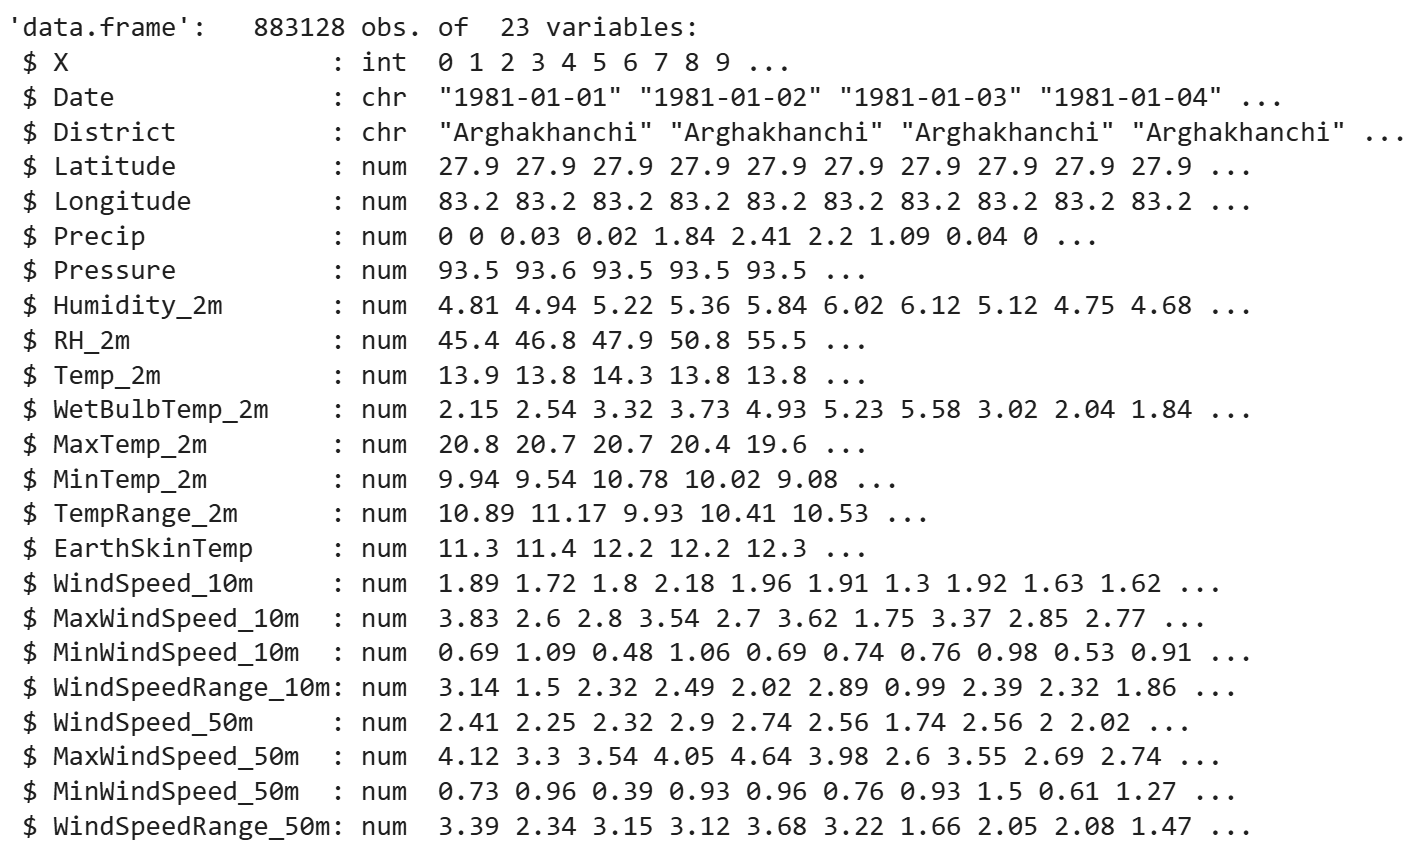
\includegraphics[width=0.7\textwidth]{figures/raw.png}
    \caption{Structure of the Climate Dataset.}
\end{figure}

\subsection{Data Summary}

The \texttt{summary()} function in R provides a quick statistical summary of each column in the dataset. It includes descriptive statistics like mean, median, minimum, maximum, and quartiles. It also shows missing values (NA) and category counts for factors.

\begin{verbatim}
summary(climate_data)
\end{verbatim}

% Figure here----------------------------
\begin{figure}[h!]
    \centering
     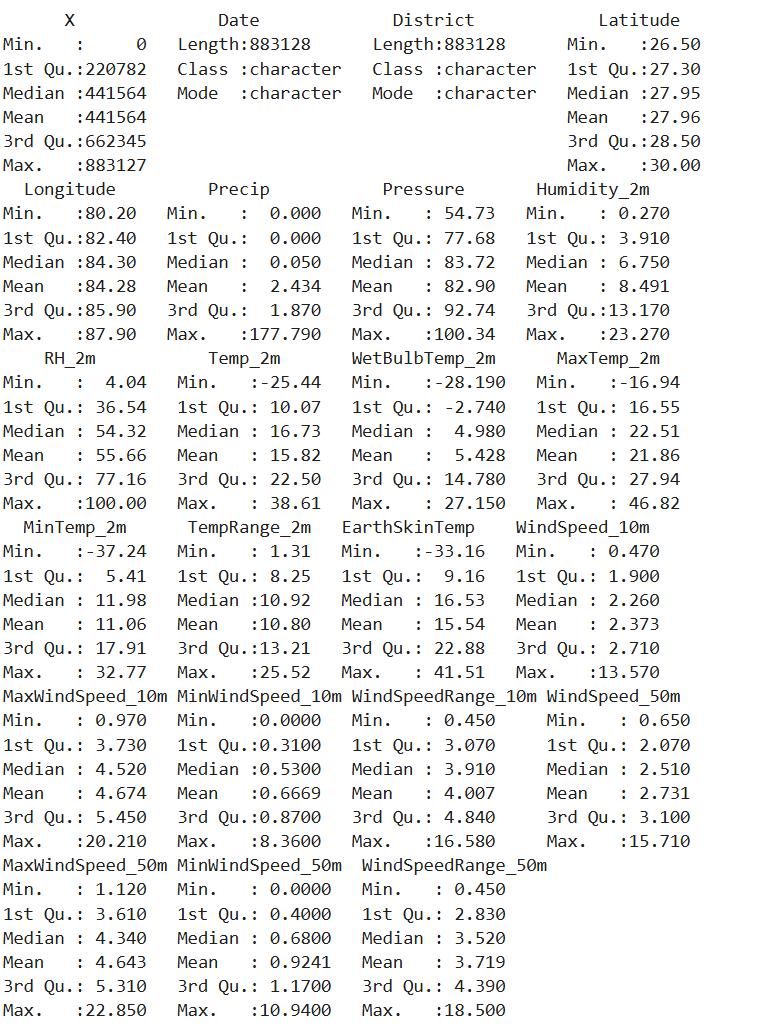
\includegraphics[width=0.5\textwidth]{figures/summary.png}
    \caption{Summary of the Climate Dataset.}
\end{figure}

\subsubsection*{What to Look for During Exploration:}

\begin{enumerate}
    \item \textbf{Data Types:} Are dates recognized as dates? Are numeric values (like temperature) stored as numbers or text?
    \item \textbf{Missing Values (NA):} How many missing values are there in each column (\texttt{summary()} is great for this)?
    \item \textbf{Ranges:} Do minimum and maximum values make sense (\texttt{summary()})? (e.g., Temperatures shouldn’t be -200°C, precipitation shouldn’t be negative).
\end{enumerate}
